
\documentclass[colorlinks=true,pdfstartview=FitV,linkcolor=blue,
            citecolor=red,urlcolor=magenta]{ligodoc}

\usepackage{graphicx}
\usepackage{amssymb}
\usepackage{amsmath}
\usepackage{longtable}
\usepackage{rotating}
\usepackage[usenames,dvipsnames]{color}
\usepackage{fancyhdr}
\usepackage{subfigure}
\usepackage{hyperref}
\ligodccnumber{T}{11}{XXXXX}{}{vX}% \ligodistribution{AIC, ISC}

\graphicspath{{images1/}}
\title{Noise Shaping in ADCs to reduce Quantization Noise in Advanced LIGO Digital Control Systems}

\author{Ayush Pandey}


\begin{document}

\section{Theory}
 The LIGO setup measures strain in the range $10^{-20}$ to $10^{-25}$ meaning that the frequency at which gravitation waves are detected in the setup currently in use is around 300 Hz. Realizing the fact that this is quite a low frequency and also since we are heaviliy concerned about any and all kinds of noises that exist in the control loop or elsewhere, Noise Shaping technique would be very useful in decreasing the noise power contributed to by the systematic noise called Quantization noise. Quantization Noise occurs both in DACs as well as ADCs and if noise shaping is implemented in both of the architectures the sensitivity of measuring the gravitational wave would be surely benefitted. 
 Noise shaping is, in essence, pushing the noise into a bandwidth which is undesired to us. As previously stated, the bandwidth of interest while detecting gravitational waves in the LIGO is in the lower ranges and the higher frequency band in undesirable. Hence, in noise shaping we push the noise spectrum to be more on the higher frequency band with respect to that in the low frequency band. This increases the SNR greatly in the desired band of frequencies. 
 
 \section{Noise Shaping in ADCs}
 Regular ADCs such as the Successive Approximation Register (SAR) ADC or the Flash ADC face the problem of aliasing which is removed by pre-filtering through an anti-aliasing filter. Aliasing is replication of the signal being converted in higher frequency range. The details of why it occurs along with its mathematical proof and its solution (the anti-aliasing filter) is explained in \cite{Oppenheim}. 
 Delta-Sigma ADCs aim to solve this problem and along with it introduce noise shaping which leads to much more simple design and increased value of SNR in the desired frequency range. It basically consists of the following stages, Oversampling, Quantization using Density of Pulses called the Sigma-Delta Modulation and finally a Decimator which reduces the output rate to frequency which can be processed further. 
 Noise shaping is achieved in Delta-Sigma ADC using feedback of the ouptut via 1-bit DAC, which is basically a switch. This feedback brings about appropriate noise shaping in the signal which shall be explained using the following block diagram.
 
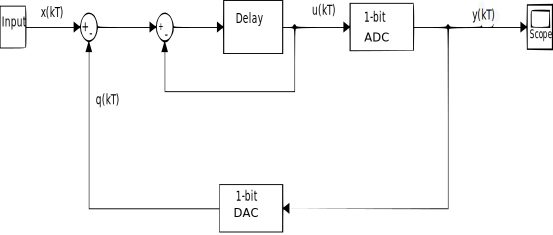
\includegraphics[scale=0.5]{Delta_Sigma_ADC_Block1}

x(kT) is the input in analog which is to be converted into digital domain and y(kT) is the output. q(kT) is the feedback signal and u(kT) is the signal which is quantized and converted to digital using the 1-bit ADC shown.
As is clear from the diagram itself that the ADC design architecture when implemented this way is very simple since it is using one bit ADC and DAC. The Delta-Sigma ADC basically trades off for much higer frequency rate over high resolution of a single converter. The 1 bit ADC may be implemented using a comparator and a 1 bit DAC is basically a switch which changes between +Vref and -Vref according to whether the output y(kT) is high or not. The reason why we have used such an architecture would be clear once we derive the effects on quantization noise it has.

\begin{equation}
u(kT)=x(kT-T)+u(kT-T)-q(kT-T)
\end{equation}
\begin{equation}
q(kT)=y(kT)
\end{equation}
The quantization error for the 1bit ADC is given by:
\begin{equation}
Q_{e}(kT)=y(kT)-u(kT)
\end{equation}
Using (1) and (3) we have,
\begin{equation}
y(kT)=x(KT-T)+u(kT-T)-q(kT-T)+Q_{e}(kT)
\end{equation}
Using (2) and (4) we have finally,
\begin{equation}
y(kT)=x(kT-T)+Q_{e}(kT)-Q_{e}(KT-T)
\end{equation}
The output of the ADC is equal to the previous input added to the difference between previous and current quantization errors. Hence, the error cancels itself which leads to better signal to noise ratio in the desired frequency range, which shall be shown by using the following block diagram (another simplified version of the previous diagram, this time signals in voltages).
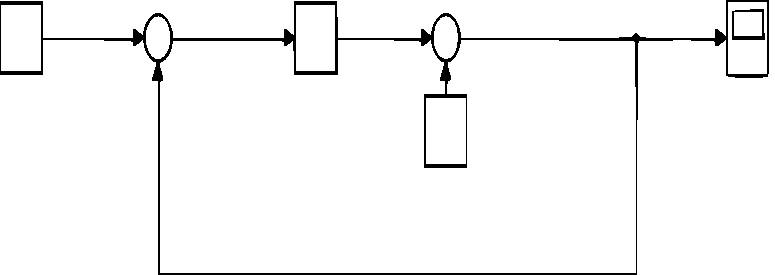
\includegraphics[scale=0.5]{Delta_Sigma_ADC_Simplified_Block}
From feedback control theory we have the following relation:
\begin{equation}
V_{out}(s)=Q_{e}(s)+\frac{V_{in}(s)-V_{out}(s)}{s}
\end{equation}

From the above equation we have:
\begin{equation}
V_{out}(s)=\frac{Q_{e}(s).s}{s+1} + \frac{V_{in}(s)}{s+1}
\end{equation}

The quantization noise is multiplied with a transfer function which represents that of a High Pass filter which essentially prooves how noise shaping takes place. The input signal is a low pass filter which is decimated (down sampled) to feed into the digital signal processor further in the control loop.

\section{Simulations in MATLAB}
The delta-sigma ADC was simulated using the Simulink tool in MATLAB.
Following is the detailed block diagram with all scopes and power spectrum measurement models shown as well: \\ \\
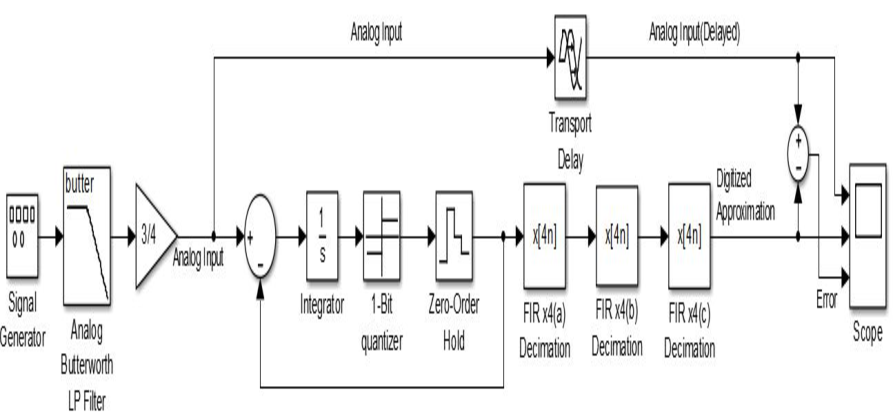
\includegraphics[scale=0.5]{Sigma_Delta_ADC_Simulink_Implementation}
The results are as follows:

Fig1. For given input, a square wave of 80Hz frequency, the following was the time domain output of the ADC. As we can see, in the last figure which represents the error, noise shaping is taking place as we described earlier mathematically. This would be further clearer from the frequency plots. \\ \\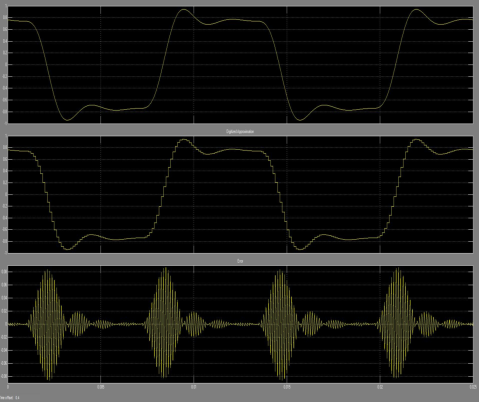
\includegraphics[scale=0.3]{ADC_Conversion_Quant_Noise_In_Time_Domain}
Fig2. The frequency spectrum of the output is shown at low frequency range (i.e. the range where signal is most prominent) and it is clear from the plot that the signal exhibits maximum maginitude in this band and falls off steeply after that. \\ \\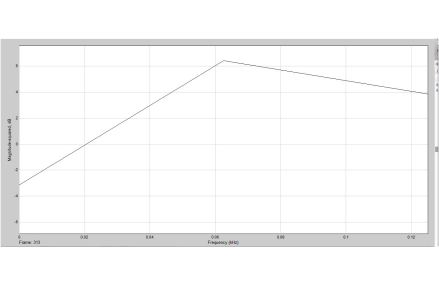
\includegraphics[scale=0.5]{Output_Spectrum_Low_Range}
Fig3. shows the frequency spectrum of the output for a wider range of frequency which further acts as evidence for the fact that the power spectrum of the outout is maximum in the desired range only. \\ \\ 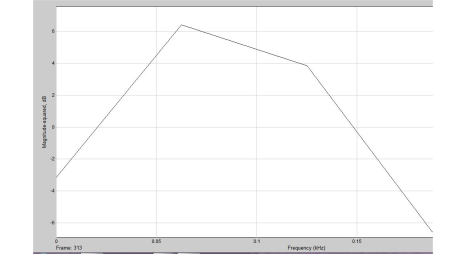
\includegraphics[scale=0.5]{Output_Spectrum_Full_Range}

Fig4. is the key figure as it shows how nicely the quantization noise is shaped, taking its lowest magnitude in the lower frequency band and rising after that and in Fig5. the full range of frequencies is showing how the quantization noise has the highest power spectrum in the undesirable (higher bandwidth) range. \\ \\ 
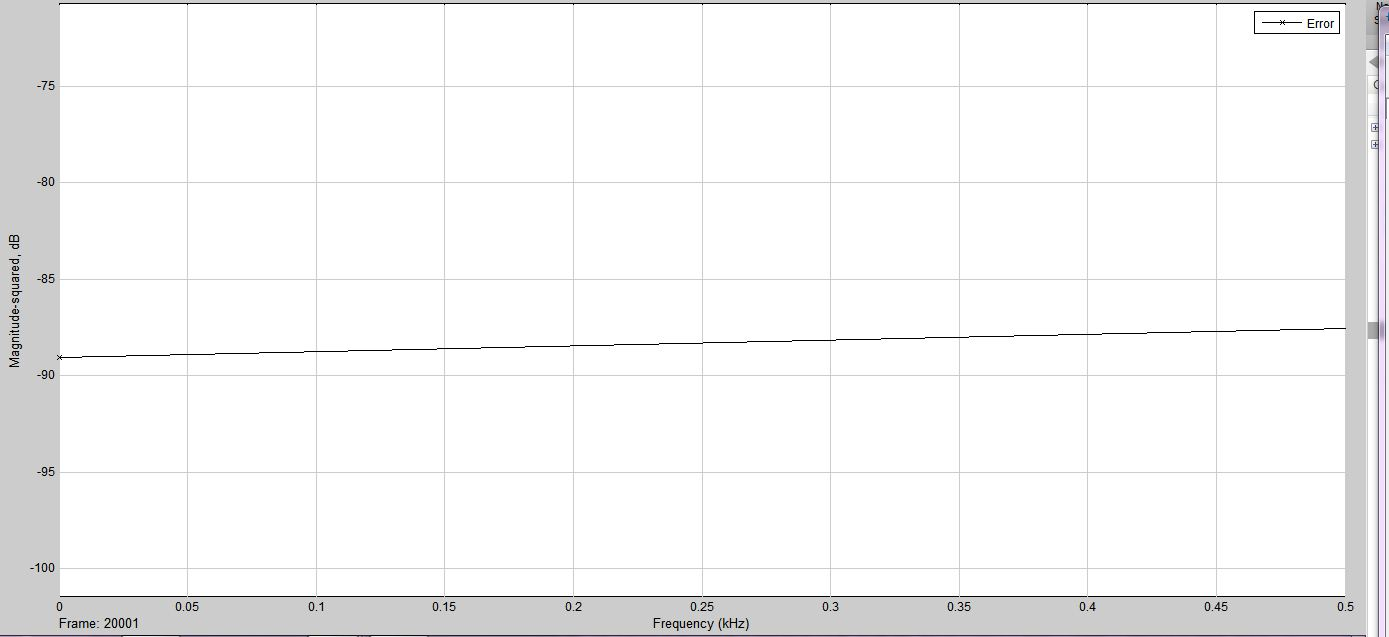
\includegraphics[scale=0.5]{Error_Frequency_Spectrum_Low_Range}

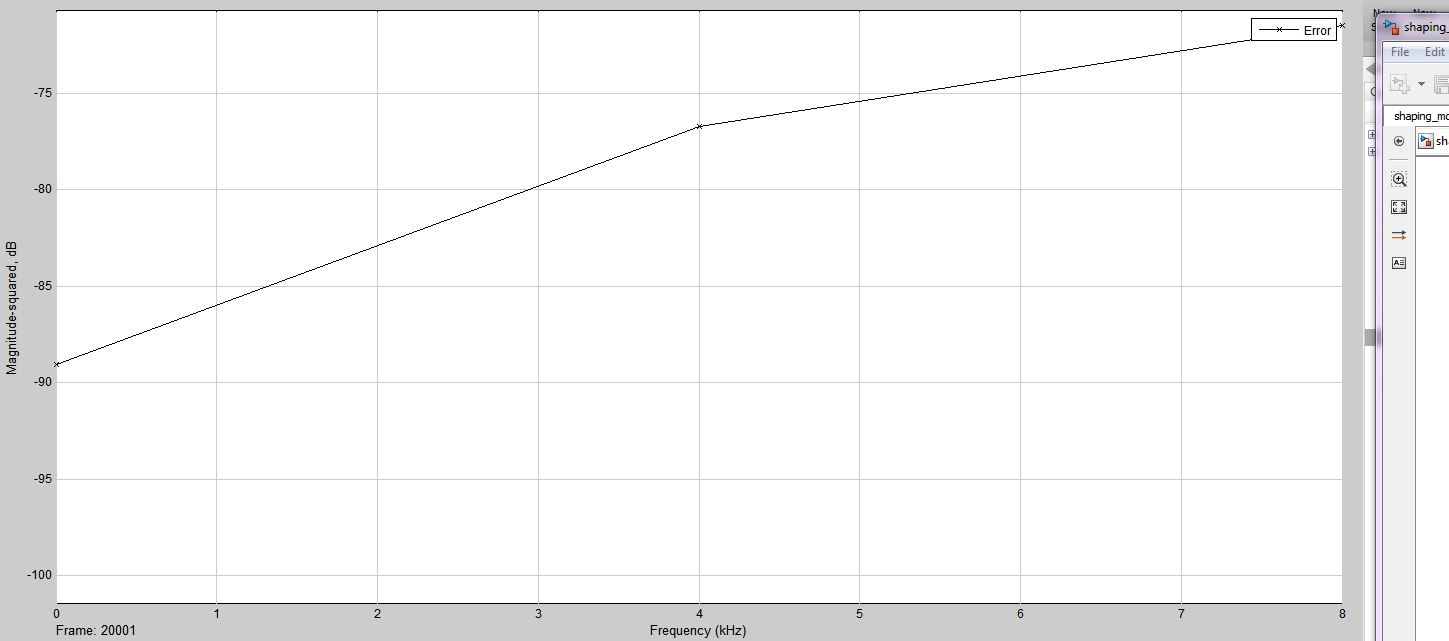
\includegraphics[scale=0.5]{Error_Frequency_Spectrum_Full_Range}


The simulink block diagram was built and compiled to get the code to implement the same. The code along with other supporting files is available at http://github.com/ayush9pandey/DACdenoising/


\begin{thebibliography}{1}  
\bibitem{Oppenheim} Oppenheim and Schafer, \emph{Discrete-Time Signal Processing}
\end{thebibliography}        
\end{document} % The document ends here
